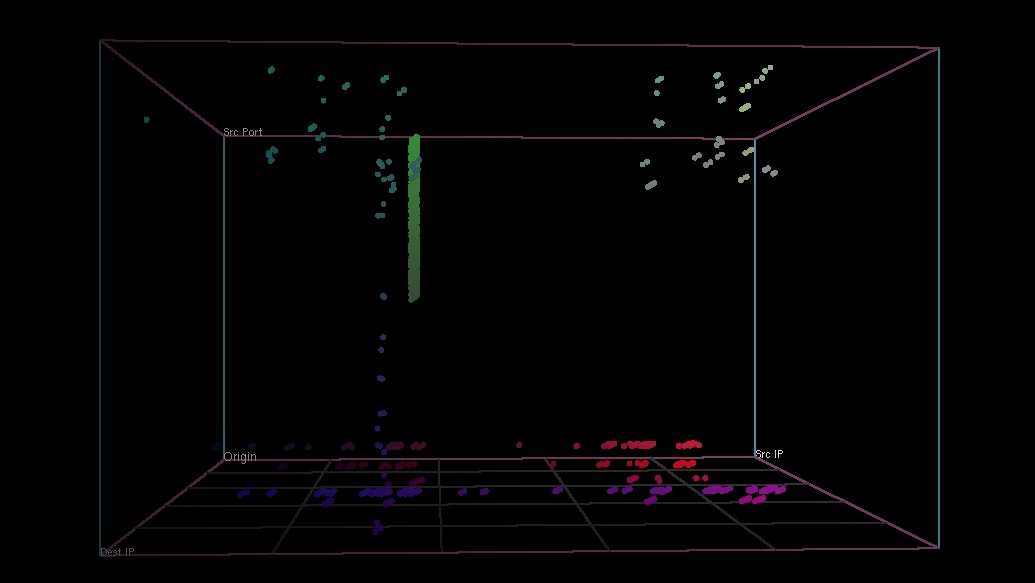
\includegraphics[width=\linewidth]{materials/cube.jpg}
The Spinning Cube is a three-dimensional scatter plot that displays packets as dots inside a rotating cube. The position of the dot is determined by its packet's attributes. This could be the combination of source port, destination port, and source IP but also any other choice of packet attributes.

The visualization is an implementation of an existing visualization tool known as the Spinning Cube of Potential Doom \cite{lau2004spinning}, but it offers additional control for the user. In particular, the axes can be chosen to represent arbitrary packet attributes.

To ensure good distinguishability of individual packets, we use the same principle of randomness as in the Data Flow visualization. Every point is animated and perturbed. In this way, multiple packets with the same attributes do not occupy the same pixel in the cube. It is thus easier to spot the packet density of an area in the cube.
